\documentclass[tikz,border=10pt]{standalone}
\usepackage{tikz}
\usetikzlibrary{positioning, arrows}
\usetikzlibrary{decorations.pathreplacing}
\usetikzlibrary{calc}
\usepackage{pgfplots}
\usepgfplotslibrary{dateplot}
\tikzset{
  font=\small,
  node distance=0.5cm and 0.2cm,
  bdata/.style={draw, rectangle, text width=2.2cm, align=center},
  sdata/.style={draw, rectangle, text width=1.75cm, align=center},
  bmodel/.style={rectangle, fill=mLightBrown, text width=4cm, align=center, rounded corners},
  smodel/.style={rectangle, fill=mLightBrown, text width=2.2cm, align=center, rounded corners},
  pred/.style={draw, rectangle, text width=1cm, align=center}
}
\usepackage{xcolor}
\definecolor{mDarkTeal}{HTML}{23373b}
\definecolor{mLightBrown}{HTML}{EB811B}
\definecolor{mDarkBrown}{HTML}{B85002}
\definecolor{mLightGreen}{HTML}{14B03D}

\usepackage{fontspec}
\setmainfont{Mona Sans}

\begin{document}
    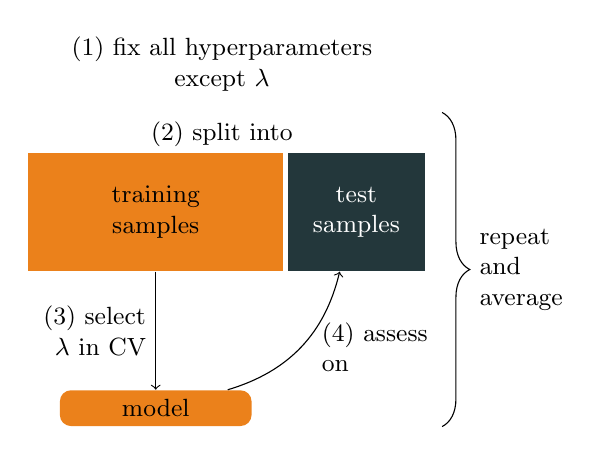
\begin{tikzpicture}[
        node distance=1cm and 0.05cm,
        trainn/.style={rectangle, text width=3cm, align=center, fill=mLightBrown, minimum height=1.5cm},
        testn/.style={rectangle, text width=1.5cm, align=center, fill=mDarkTeal, text=white, minimum height=1.5cm},  
        fixn/.style={rectangle, text width=4.7cm, align=center},
        splitn/.style={rectangle, text width=4.5cm, align=center}
        ]
        \node[trainn] (traindata) {training\\ samples};
        \node[testn, right=of traindata] (testdata) {test samples};
        \node[splitn, above=0.7cm of $(traindata)!0.33!(testdata)$] (split) {(2) split into};
        \node[fixn, above=0.15cm of split] (fixhyper) {(1) fix all hyperparameters\\ except $\lambda$};
        \node[smodel, below=1.5cm of traindata] (model) {model};
        
        \draw[->] (traindata) -- node[midway, left, align=right] {(3) select\\ $\lambda$ in CV} (model);
        \draw[->] (model) to[bend right] node[midway, right=4pt, align=left] {(4) assess\\ on} (testdata);

        \path let \p1 = (split.east) in \pgfextra{\xdef\bracex{\x1}};
        \path let \p1 = (split.north) in \pgfextra{\xdef\braceuy{\y1}};
        \path let \p1 = (model.south) in \pgfextra{\xdef\bracely{\y1}};
        \draw[decorate,decoration={brace,amplitude=10pt,mirror,raise=12pt}] 
        (\bracex, \bracely) -- (\bracex, \braceuy) node[midway, right=22pt, align=left] {repeat\\ and\\ average};
    \end{tikzpicture}
\end{document}